\subsection*{Checkpoint 1.18: Evaluating Trigonometric Functions}

\subsubsection*{Instruction}

\begin{enumerate}[label=(\alph*)]
  \item
    Evaluate $ cos(3\pi/4) $.
  \item
    Evaluate $ sin(-\pi/6) $.
\end{enumerate}

\subsubsection*{Solution}

\begin{enumerate}[label=(\alph*)]
  \item
    We start by sketching an unit circle with the angle $ 3\pi/4 $, see figure \ref{figure:checkpoint-1.1.18-a-1}. We know that $ cos(3\pi/4) $ is defined to be the $ x $-coordinate of the point sketched on the unit circle.

    \begin{figure}[H]
      \centering
      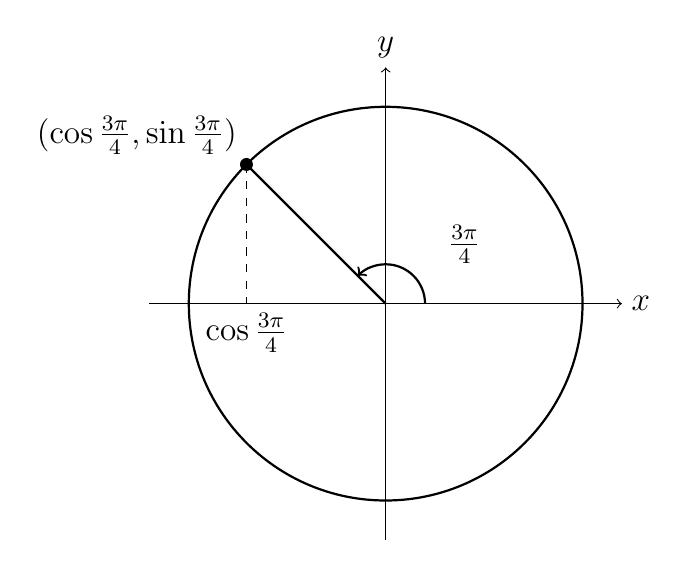
\begin{tikzpicture}[scale=2.5, font=\large]
        % Define angle in degrees
        \pgfmathsetmacro{\angle}{135}
        \pgfmathsetmacro{\x}{cos(\angle)}
        \pgfmathsetmacro{\y}{sin(\angle)}

        % Draw the unit circle
        \draw[thick] (0,0) circle(1);

        % Axes
        \draw[->] (-1.2,0) -- (1.2,0) node[right] {$x$};
        \draw[->] (0,-1.2) -- (0,1.2) node[above] {$y$};

        % Point at 3π/4
        \draw[thick] (0,0) -- (\x,\y);
        \filldraw (\x,\y) circle(0.03) node[above left] {$(\cos \frac{3\pi}{4}, \sin \frac{3\pi}{4})$};

        % Cosine projection
        \draw[dashed] (\x,\y) -- (\x,0) node[below] {$\cos \frac{3\pi}{4}$};

        % Angle marking
        \draw[thick,->] (0.2,0) arc[start angle=0,end angle=\angle,radius=0.2];
        \node at (0.4,0.3) {$\frac{3\pi}{4}$};

      \end{tikzpicture}
      \caption{Unit circle with point at angle $ 3\pi/4 $}
      \label{figure:checkpoint-1.1.18-a-1}
    \end{figure}

    There is a table with cosine values in given in the book that this exercise is taken from, but it only covers values from the first quadrant and our angle is in the third quadrant. But we can find the supplementary angle to our angle that will be $ \pi - 3\pi/4 = \pi/4 $ as shown in figure \ref{figure:checkpoint-1.1.18-a-2}.

    \begin{figure}[H]
      \centering
      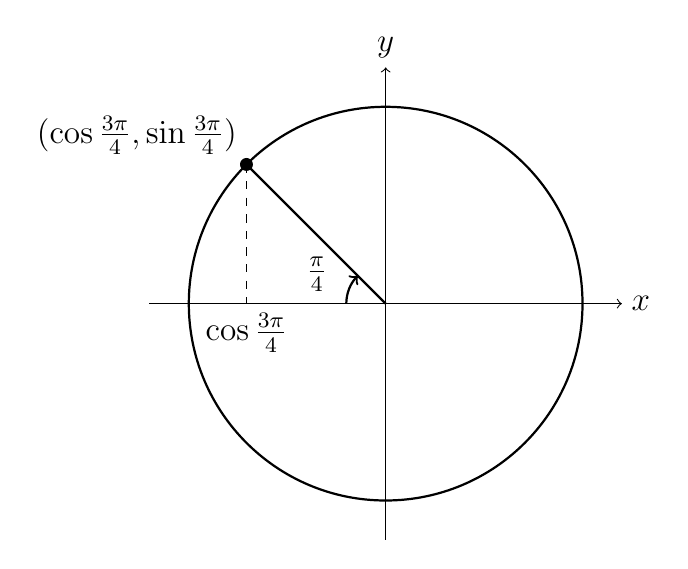
\begin{tikzpicture}[scale=2.5, font=\large]
        % Draw the unit circle
        \draw[thick] (0,0) circle(1);

        % Axes
        \draw[->] (-1.2,0) -- (1.2,0) node[right] {$x$};
        \draw[->] (0,-1.2) -- (0,1.2) node[above] {$y$};

        % Angle 3π/4 (135 degrees)
        \draw[thick] (0,0) -- (-0.7071,0.7071);
        \filldraw (-0.7071,0.7071) circle(0.03) node[above left] {$(\cos \frac{3\pi}{4}, \sin \frac{3\pi}{4})$};

        % Draw the cosine value as a horizontal projection
        \draw[dashed] (-0.7071,0.7071) -- (-0.7071,0) node[below] {$\cos \frac{3\pi}{4}$};

        % Mark the opposite angle of 3pi/4 rad
        \draw[thick,->] (-0.2,0) arc[start angle=180,end angle=135,radius=0.2];
        \node at (-0.35, 0.15) {$\frac{\pi}{4}$};

      \end{tikzpicture}
      \caption{Unit circle with point at the supplementary angle $ \pi/4 $}
      \label{figure:checkpoint-1.1.18-a-2}
    \end{figure}

    We know from the table of cosine values given in the book that $ cos(\pi/4) = \sqrt{2}/2 $. It follows that we value that we are looking for will be the same but negative since our angle is mirrored in the $y$-axle. We conclude that $ cos(3\pi/4) $ equals $ -\sqrt{2}/2 $.
  \item
    We start by sketching an unit circle with the angle $ -\pi/6 $, see figure \ref{figure:checkpoint-1.1.18-b}. We know that $ sin(-\pi/6) $ is defined to be the $ y $-coordinate of the point sketched on the unit circle.

    \begin{figure}[H]
      \centering
      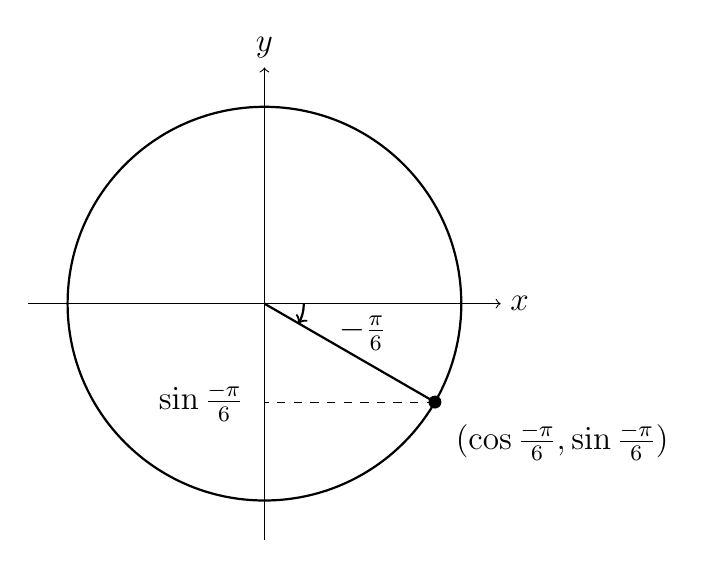
\begin{tikzpicture}[scale=2.5, font=\large]
        % Define angle in degrees
        \pgfmathsetmacro{\angle}{-30} % -pi/6 = -30 degrees
        \pgfmathsetmacro{\x}{cos(\angle)}
        \pgfmathsetmacro{\y}{sin(\angle)}

        % Draw the unit circle
        \draw[thick] (0,0) circle(1);

        % Axes
        \draw[->] (-1.2,0) -- (1.2,0) node[right] {$ x $};
        \draw[->] (0,-1.2) -- (0,1.2) node[above] {$ y $};

        % Draw angle line
        \draw[thick] (0,0) -- (\x,\y);
        \filldraw (\x,\y) circle(0.03)
        node[below right, xshift=4pt, yshift=-4pt]
        {$(\cos \frac{-\pi}{6}, \sin \frac{-\pi}{6})$};

        % Dashed projection to the y axis
        \draw[dashed] (\x,\y) -- (0,\y) node[left, xshift=-4pt]
        {$\sin \frac{-\pi}{6}$};

        % Angle marking (clockwise)
        \draw[thick,->] (0.2,0) arc[start angle=0, end angle=\angle, radius=0.2];
        \node at (0.5,-0.15) {$-\frac{\pi}{6}$};

      \end{tikzpicture}
      \caption{Unit circle with point at angle $ -\pi/6 $}
      \label{figure:checkpoint-1.1.18-b}
    \end{figure}

    There is a table in the book with some common sinus values. The value for $ sin(-\pi/6) $ is not in the table but it is stated in the table that $ sin(\pi/6) = 1/2 $. This value is related to the value we are looking for, difference being that our value is mirrored in the $x$-axis. The answer is hence the additive inverse, $-1/2$.
\end{enumerate}

\subsubsection*{Answer}

\begin{enumerate}[label=(\alph*)]
  \item
    $ cos(3\pi/4) = -\sqrt{2}/2 $.
  \item
    $ sin(-\pi/6) = -1/2 $.
\end{enumerate}
